% -*- TeX-master: "report" -*-

\section{Complex Predicates}
\label{sec-complex-preds}
%         *         *         *         *         *         *        80 columns |
A complex predicate $C$ is defined as $C = \phi(p_1, p_2, \ldots p_k)$ where 
$p_1, p_2, \ldots p_k$ are simple predicates and $\phi$ is a function in 
conjunctive normal form (CNF).  Evaluating $C$ requires combining predicates 
using $\wedge$ (``and'') and $\vee$ (``or''); a negation operator is not required 
because by design, the negation of every CBI predicate $p$ is also a predicate.  
For $N$ predicates there are $2^{2^N}$ such Boolean functions 
\cite{MathWorld:BoolFuncs}.  There may be hundreds of simple predicates involved 
in the analysis, and so this a prohibitively large number.

To reduce complexity we consider only functions of two predicates.  Out of the
16 ($2^{2^2}$) such functions, we consider only conjunction and disjunction since
they are likely to be most easily understood by programmers.  Our revised
definition is $C = \phi(p_1, p_2)$ where $\phi \in \{\vee, \wedge\}$.  Conjunction
and disjunction are commutative, and the reflexive cases ($p_1 \wedge p_1$ and 
$p_1 \vee p_1$) are uninteresting.  This reduces the number of complex predicates
to just ${N \choose 2} = \frac{N (N-1)}{2}$ binary conjunctions and an equal number 
of binary disjunctions.  These may be evaluated for a set of $R$ runs in $O(R N^2)$ 
time.  The revised definition for a complex predicate is used throughout; related
definitions may be trivially extended to the general case.

\subsection{Measuring Complex Predicates}
\label{sec-measuring}

For a predicate $p$ and a run $R$, $R(p) = \true$ if and only if $p$ was observed to be true at least once during run $R$.  Similarly we could define $R(C)$ as follows:
\begin{defn}
\label{dfn1}
For a complex predicate $C = \phi(p_1, p_2)$, $R(C) \equiv \true$ iff at some point during the execution of the program, $C$ was observed to be true.
\end{defn}

The difficulty with this notion of complex predicates is that $C$ must be explicitly monitored during the program execution.  For example, if $C_1 = p_1 \wedge p_2$ then $R(p_1) = \true$ and $R(p_2) = \true$ does not imply that $R(C) = \true$.  $p_1$ and $p_2$ may be true at different stages of execution but never true at the same time.  Furthermore, when $p_1$ and $p_2$ appear at different source locations, there may be no single point in time at which both are even well-defined and therefore simultaneously observable.  In order to be able to estimate the value of $C$ from its components, we adapt a less time-sensitive definition as follows:
\begin{defn}
\label{dfn2}
For a complex predicate $C = \phi(p_1, p_2)$, $R(C) = \true$ iff $\phi(R(p_1), R(p_2)) = \true$
\end{defn}

In other words, we assume that $R$ is distributive over $\phi$, effectively removing the requirement that all $p_i$ be observed simultaneously.  This can lead to false positives, because $R(C)$ may be computed to $\true$ when it is actually $\false$ at all moments in time.  False negatives, however, cannot arise.  The impact of this assumption on the score of $C$ may be either positive or negative depending on whether $R$ failed or succeeded.

\subsection{Three Valued Logic}
\label{sec-tvl}
This section explains how conjunctions and disjunctions are actually computed.  Three-valued logic is used because the value of a predicate in a run may not be certain. This can arise in two situations:
\begin{enumerate}
\item The predicate was not observed in a run because the run did not reach the line where it was defined.
\item The program reached the line where the predicate was defined but was not observed because of sampling.
\end{enumerate}

In such a case, the value of a predicate $p$ is considered unknown.  For the analysis introduced in \autoref{sec-bground}, it is enough to consider whether $R(p)$ was $\true$ or $\neg \true$ (either $\false$ or $\unknown$), since $\obs{R}{p}$ is used independently.  When constructing conjunctive predicates, however, considering the sub-cases of $\neg \true$ separately allows additional run information to be derived.

Consider a complex predicate $C = p_1 \wedge p_2$.  If either $R(p_1)$ or $R(p_2)$ was $\false$ in a run $R$, then $R(C) = \false$ - one false value is sufficient to disprove a conjunction.  If both $R(p_1)$ and $R(p_2)$ were $\true$, then $C$ was observed to be true.  Otherwise, the value of $R(C)$ is $\unknown$. This is shown using a three-valued truth table in \autoref{tab:and}.  The emphasized entries would have been $\unknown$ if the subcases of $\neg \true$ were treated as equivalent.  This increases the number of runs where a conjunctive predicate is considered to be observed, affecting its $\Importance$ score.

Similarly one true value is sufficient to prove a disjunction.  While the distinction between $\false$ and $\unknown$ is less important when constructing a disjunctive predicate, the same style of short-circuit evaluation is used.  The truth table for complex predicate $D = p_1 \vee p_2$ is shown in \autoref{tab:or} for completeness.

\begin{table}
  \caption{3-valued Truth Table for $C = p_1 \wedge p_2$}
  \label{tab:and}
  \centering
  \begin{tabular}{c|ccc}
    % after \\: \hline or \cline{col1-col2} \cline{col3-col4} ...
    $p_1 \diagdown p_2$ & T & F & ? \\
    \hline
    T & T & F & ? \\
    F & F & F & \emph{F} \\
    ? & ? & \emph{F} & ? \\
  \end{tabular}
\end{table}


\begin{table}
  \caption{3-valued Truth Table for $D = p_1 \vee p_2$}
  \label{tab:or}
  \centering
  \begin{tabular}{c|ccc}
    % after \\: \hline or \cline{col1-col2} \cline{col3-col4} ...
    $p_1 \diagdown p_2$ & T & F & ? \\
    \hline
    T & T & T & T \\
    F & T & F & ? \\
    ? & T & ? & ? \\
  \end{tabular}
\end{table}

\subsection{Interesting Complex Predicate}
Even using the revised definition for $C$ the number of complex predicates is still quadratic in the number of simple predicates.  A large number of complex predicates formed by this procedure are likely to be useless in the analysis of the program.  A complex predicate that has a lower score than one of its components is useless.  The component (simple) predicate with a higher score is a better predictor of failure, and so the complex predicate adds nothing to the analysis.

\begin{defn}
\label{dfn3}
A complex predicate $C = \phi(p_1, p_2)$ is ``interesting'' iff $\Importance(C) > \max(\Importance(p_1), \Importance(p_2))$
\end{defn}

In the case where the complex predicate has the same score as a component predictor, the simpler one is preferable.  Keeping only interesting combinations of predicates reduces the memory burden of storing them, and helps ensure the utility of a complex predicate that is presented to the user.

\subsection{Pruning}
\label{sec-pruning}
Constructing complex predicates from simple ones requires generating two bits of information (according to the three value logic discussed in \autoref{sec-tvl}) for each program run; as CBI is meant to analyze deployed software program runs potentially number in the hundreds of thousands, if not millions.  The measure of a complex predicate's relevance to a bug is its $\Importance$ score, which can only be derived once run information has been generated.  Complex predicates with low $\Importance$ provide no information useful in debugging and are not presented to the programmer; in such a case the effort to form the predicate has been wasted.  This provides the motivation to prune combinations before run information is generated based on an estimate of their resulting scores.  If this estimate falls below the threshold required for the predicate to be presented to the programmer, the complex predicate is not constructed.  Pruning predicates before they are constructed reduces a $O(R)$ operation (constructing run information) to one which executes in constant time.

The threshold $\Importance$ value, which complex predicates must potentially exceed to be constructed, can be calculated in two ways:
\begin{enumerate}
\item Only \emph{interesting} complex predicates are retained; for predicate $C = \phi(p_1, p_2)$ the threshold is max($\Importance(p_1)$, $\Importance(p_2)$).
\item During redundancy elimination, only the predicate with the highest score is retained at each iteration.  The threshold is therefore the highest score yet seen (including those of simple predicates).
% Note: as of 12/06 our implementation didn't do this.  This may have changed with recent modifications...
\end{enumerate}

Using an upper bound as the estimate of $\Importance$ guarantees that no predicate is pruned erroneously.  This upper bound can be determined by maximizing $F(p)$ and $\Increase(p)$ under constraints based on the propositional operation.  $\Importance(P)$ (\autoref{eqn2}), being a harmonic mean of these two terms, will likewise be maximized.

In this context, the disjunction $D = p_1 \vee p_2$ can be considered as the union of the set of runs where $p_1$ was $\true$ and the set where $p_2$ was $\true$.  The size of the resulting set is maximized when the two do not overlap, and that is the assumption made when calculating an upper bound on $F(D)$.  $S(D)$ is minimized by making the opposite assumption - that one is a subset of the other.  The size of the union is thus the size of the superset.  The best disjunction that can be formed using $p_1$ and $p_2$ will have the following parameters:

\begin{eqnarray*}
  F(D)' &=&  F(p_1) + F(p_2) \\
  S(D)' &=&  \max(S(p_1),S(p_2)) \\
  \obs{F}{D}' &=& 0 \\
  \obs{S}{D}' &=& S(D)'
\end{eqnarray*}

The second term in $\Increase$ (\autoref{eqn1}) can only reduce the result, and so it is ignored in calculating an upper bound.  For completeness, $\obs{S}{D}'$ is assigned the same value as $S(D)'$ even though it does not affect $\Increase(D)$.  The $F(D)$ component of $\Importance$ is maximized while maximizing $\Increase$.  Thus the $\Importance$ score calculated with the above values is an upper bound on the score of the disjunction of $p_1$ and $p_2$. As a concrete example, suppose $F(p_1) = 500$, $F(p_2) = 1000$, $S(p_1) = 250$ and $S(p_2) = 500$. Furthermore assume the total number of failed runs is 1500. To maximize the value of $\Importance(D)$ where $D = p_1 \vee p_2$,  we will let $F(D)' = 500 + 1000 = 1500$, $S(D)' = 500$. As a result, the upper bound of $\Increase(D)$ will be $\frac{1500}{2000}=0.75$ when we disgard the term after the minus sign in \autoref{eqn2}. Finally the upper bound of $\Importance(D)$ would be $\frac{2}{\frac{1}{0.75}+\frac{1}{log1500/log1500}} = 0.856$. 

The conjunction $C = p_1 \wedge p_2$ can be regarded as the intersection of the set of runs where $p_1$ was $\true$ and the set where $p_2$ was $\true$.  Maximizing $F(C)$ requires that one of the intersecting sets is a subset of the other, making the size of the intersection the size of the smaller set.  A minimal $S(C)$ is found when the component sets are non overlapping; the intersection of two such sets is empty.

\begin{eqnarray*}
  F(C)' &=&  \min(F(p_1),F(p_2)) \\
  S(C)' &=& 0
\end{eqnarray*}

If the second term in $\Increase$ is ignored, as with disjunctions, the upper bound of a conjoined predicate's $\Increase$ score is 1.  This is the maximum $\Increase$ possible, reducing the likelihood of a conjoined predicate being pruned to almost zero.  The second term is therefore used for conjunctions to drop the upper bound to a more useful level. To minimize the second term, we are going to minimize $\obs{F}{C}$ and maximize $\obs{S}{C}$.

$\obs{F}{C}$ is minimized by assuming that $C$ was \textit{observed} only in the (failed) runs where it was true.  Maximizing $\obs{S}{C}$ is more difficult.  Recall that a conjunction can be considered \textit{observed} if either component is \textit{observed false}, or both are \textit{observed true}.  The combination of successful runs where a predicate is \textit{observed false} (union) is maximized if the sets are non overlapping, while the combination where they are \textit{observed true} (intersection) is maximized if one is a subset of the other.  By assuming both cases meet that criteria $\obs{S}{C}$ can be maximized.  Its value is the sum of successful runs where $p_1$ was \textit{observed} and those where $p_2$ was \textit{observed false}, formed as the difference between $\obs{S}{p_2}$ and $S(p_2)$.  \autoref{maxsuccess} depicts the above scenario which maximizes $\obs{S}{C}$: notice that the sets $S(\neg p_1)$ and $S(\neg p_2)$ are disjoint and $s(p_1)$ is a subset of $s(p_2)$.  Since the result may differ depending on which predicate is chosen as $p_1$, the larger result is used.
\begin{eqnarray*}
  \obs{F}{C}' &=& F(C)' \\
  \obs{S}{C}' &=&
  \max(\obs{S}{p_1} + \obs{S}{p_2} - S(p_2),\\
  & &\ \ \ \ \obs{S}{p_2} + \obs{S}{p_1} - S(p_1))
\end{eqnarray*}

\begin{figure}[h]
  \centering
  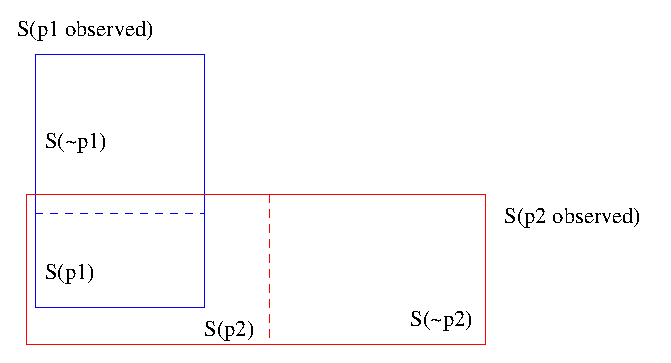
\includegraphics[scale = 0.6]{charts/maxsuccess}
  \caption{Maximizing \obs{S}{C}}
  \label{maxsuccess}
\end{figure}

Pruning complex predicates using the above calculations reduces the computational intensity of the analysis without affecting the results.  The effectiveness of pruning is examined in \autoref{sec-effectprune}.
